% Provenance (never printed): see sources/outline_sources.md (Year 3:
% energy-balance models, the one-layer model recalled; ice-albedo feedback
% and multiple equilibria; how general circulation models are built and
% evaluated).
% Brief: sources/book5/BRIEFS.md, ch. 22. Curves from
% figdata/bachelor-3/budyko_sellers.py (the zero-dimensional model and
% Budyko's latitudinal model; the brief's ebm_0d is folded into it) and
% two_layer.py. Exercise and problem values in the Book 5 scratch calculator
% calc/ch22.py. The model planet, model X and the ensemble of exercise 12 are
% invented.
\chapter{Modelos climáticos}\label{ch:b3:climate-models}

Tome a luz solar que chega à Terra, \qty{340}{W/m^2} em média sobre o
globo, e uma lei para o infravermelho que ela devolve ao espaço, ajustada a
trinta anos de uma reanálise das observações. Suponha-se que o albedo do planeta suba do valor do
solo descoberto e do mar até o do gelo, à medida que a superfície esfria. Equilibrando os dois
fluxos, a equação tem três soluções: um planeta a
\qty{14}{\celsius}, próximo da média do real; um planeta a
\qty{8}{\celsius}; e um planeta a \qty{-46}{\celsius}, congelado de polo a
polo. Os modelos climáticos, desde essas poucas linhas até programas executados nos maiores
computadores, são ferramentas para perguntar qual clima um dado planeta tem, como ele
chega até lá e como muda quando seu balanço de energia é perturbado.
% ledger: nasa:solar-mean, data:b5-ncep-air, data:b3-ncep, budyko69:albedo

\begin{recall}
O corpo negro, a lei de Stefan--Boltzmann, o efeito estufa e o
modelo de uma camada da atmosfera estão nos livros de física; o albedo e
o balanço de energia da Terra, nos livros escolares. A radiação de onda longa
emitida para o espaço, a temperatura de emissão e o transporte meridional de calor estão
no volume do primeiro ano, no seu capítulo sobre radiação e transporte de calor. A
retroalimentação gelo--albedo e a Terra bola de neve estão no volume do segundo ano, no
seu capítulo sobre a Terra pré-cambriana; o forçamento radiativo efetivo, o
parâmetro de retroalimentação climática $\lambda < 0$, a sensibilidade climática de equilíbrio
(ECS) e a resposta climática transiente (TCR) no seu capítulo
sobre mudança climática antropogênica; a previsão numérica do tempo e a
previsão por conjunto no seu capítulo sobre sistemas meteorológicos. As equações de
movimento na Terra em rotação, com a \omterm{def:b3:gfd-foundations:hydrostatic}{aproximação hidrostática}, estão no
Capítulo~\ref{ch:b3:gfd-foundations}.
\end{recall}

\section{O balanço de energia de um planeta}\label{sec:b3:climate-models:zero-d}

Em média sobre a esfera e ao longo de um ano, cada metro quadrado no topo
da atmosfera recebe $Q = S_0/4 = \qty{340}{W/m^2}$, um quarto da
irradiância solar $S_0 = \qty{1360}{W/m^2}$. Uma fração $\alpha$, o
albedo planetário, é refletida; o restante, $Q(1 - \alpha)$, é absorvido e
deve ser devolvido ao espaço como infravermelho. Um corpo negro emitiria $\sigma
T^4$; a radiação de onda longa emitida pela Terra (OLR, do inglês \textit{outgoing longwave radiation}) é menor, por causa do
efeito estufa e, na faixa de temperaturas de superfície encontradas na
Terra, ela é próxima de uma reta,
\[
\text{OLR} = A + BT ,
\]
com $T$ a temperatura da superfície em graus Celsius. Em 1969, Budyko ajustou
essa lei à radiação emergente calculada para 260 estações, com uma correção para
a nebulosidade $n$: $I = a + bT - (a_1 + b_1T)n$, $a = 14.0$, $b = 0.14$, $a_1 =
3.0$ e $b_1 = 0.10$ em \unit{kcal.cm^{-2}} por mês, com dispersão abaixo de
\qty{5}{\percent}. Para uma nebulosidade média de 0.5, isso dá $A =
\qty{199}{W/m^2}$ e $B = \qty{1.43}{W.m^{-2}.\celsius^{-1}}$. As
médias zonais anuais da Reanálise~1 do NCEP--NCAR para 1991--2020, ponderadas pela área,
dão $A = \qty{211.9}{W/m^2}$ e $B = \qty{1.816}{W.m^{-2}.\celsius^{-1}}$,
com dispersão de \qty{10}{W/m^2} em torno da reta. Esses valores são usados
a seguir.
% ledger: nasa:solar-mean, budyko69:olr, data:b5-ncep-air, data:b3-ncep

\begin{definition}[Modelo de balanço de energia]\label{def:b3:climate-models:ebm}
Um \emph{modelo de balanço de energia}\index{modelo de balanço de energia} é um modelo climático
que calcula uma temperatura de superfície --- uma única média global ou uma
média sobre cada latitude --- a partir do balanço da luz solar absorvida, do
infravermelho emitido para o espaço e, se a temperatura depende da latitude, do
calor transportado em direção aos polos. Em sua forma de dimensão zero,
\[
C\,\frac{\mathrm dT}{\mathrm dt} = Q\big(1 - \alpha(T)\big) - (A + BT) ,
\]
em que $C$ é a capacidade térmica por unidade de área da parte do sistema que
se aquece junto com a superfície.
\end{definition}

Com $\alpha = 0.30$, o equilíbrio é $T = (238 - 211.9)/1.816 =
\qty{14.4}{\celsius}$; a média de área da reanálise é
\qty{14.2}{\celsius}. Um forçamento $F$, como o de uma variação do
dióxido de carbono, soma-se ao lado direito. Próximo de um equilíbrio, a resposta é
governada pelo parâmetro de retroalimentação climática $\lambda$ do volume do segundo ano:
com o albedo fixo, $\lambda = -B$.
% ledger: earth:albedo, data:b5-ncep-air

\begin{theorem}[Tempo de resposta de um clima de uma caixa]\label{thm:b3:climate-models:response}
Suponha-se que um clima esteja em equilíbrio e que um forçamento constante $F$ seja
ligado em $t = 0$. Se o desvio $T'$ em relação ao equilíbrio obedece a $C\,\mathrm
dT'/\mathrm dt = F + \lambda T'$, com $C > 0$ e $\lambda < 0$ constantes,
então
\[
T'(t) = -\frac{F}{\lambda}\Big(1 - \mathrm e^{-t/\tau}\Big), \qquad
\tau = -\frac{C}{\lambda} .
\]
O novo equilíbrio é $-F/\lambda$, e o clima percorre a fração $1
- \mathrm e^{-1} = \num{0.63}$ do caminho no tempo $\tau$.
\end{theorem}

\begin{proof}
$T'_\infty = -F/\lambda$ anula o lado direito. A diferença
$u = T' - T'_\infty$ obedece a $C\,\mathrm du/\mathrm dt = \lambda u$, logo $u =
u(0)\,\mathrm e^{\lambda t/C}$, com $u(0) = F/\lambda$.
\end{proof}

A capacidade térmica que importa ao longo de alguns anos é a do oceano superior.
O emulador de duas camadas do sexto relatório de avaliação do
Painel Intergovernamental sobre Mudança do Clima (IPCC), calibrado em 44 modelos climáticos,
fornece para a camada superficial $C = \qty{8.1}{W.yr.m^{-2}.\celsius^{-1}}$, a capacidade térmica
de uma camada de água do mar de \qty{62}{m} de profundidade. Com $\lambda = -B$, o
tempo de resposta é $8.1/1.816 = \num{4.5}\text{ anos}$. O clima real também aquece
o oceano profundo, muito mais lentamente; a Seção~\ref{sec:b3:climate-models:two-layer}
acrescenta esse efeito.
% ledger: ar6sm7:two-layer, teos10:cp0, data:b5-ncep-air

\section{Gelo, albedo e equilíbrios múltiplos}\label{sec:b3:climate-models:multiple}

A retroalimentação gelo--albedo do volume do segundo ano faz o albedo depender da
temperatura. Considere-se $\alpha = 0.62$ para um planeta cuja superfície esteja abaixo de
$T_I = \qty{-10}{\celsius}$, o albedo do gelo no modelo de Budyko, $\alpha
= 0.30$ acima de $T_F = \qty{+10}{\celsius}$, e uma reta entre eles, à medida que
o gelo recua. A rampa é uma escolha deste capítulo; qualquer albedo que
aumente à medida que o planeta esfria produz o mesmo quadro.
% ledger: budyko69:albedo, earth:albedo

\begin{definition}[Múltiplos equilíbrios climáticos; bifurcação sela-nó]\label{def:b3:climate-models:multiple-equilibria}
Um modelo climático tem \emph{múltiplos equilíbrios climáticos}\index{múltiplos equilíbrios climáticos}
quando, para as mesmas condições externas, possui mais de
um estado estacionário. Um equilíbrio é estável se um pequeno afastamento
dele decai, instável se cresce. Uma \emph{bifurcação
sela-nó}\index{bifurcação sela-nó} é o valor de um parâmetro no qual
um equilíbrio estável e um instável se encontram e desaparecem juntos.
\end{definition}

\begin{proposition}[Três equilíbrios e sua estabilidade]\label{prop:b3:climate-models:three}
Escreve-se $N(T) = Q(1 - \alpha(T)) - (A + BT)$ para o fluxo descendente líquido. Um
equilíbrio $T^*$, $N(T^*) = 0$, é estável se $N'(T^*) < 0$ e instável se
$N'(T^*) > 0$. Com a rampa acima, $N' = -B$ nos ramos de bola de neve e
sem gelo, que são estáveis onde existem, e $N' = -B -
Q\,\mathrm d\alpha/\mathrm dT$ na rampa, que é instável quando $Q\,
|\mathrm d\alpha/\mathrm dT| > B$. Para $Q = \qty{340}{W/m^2}$ o modelo tem
três equilíbrios, \qty{-45.5}{\celsius} (estável), \qty{7.8}{\celsius}
(instável) e \qty{14.4}{\celsius} (estável).
\end{proposition}

\begin{proof}
Perto de $T^*$, $C\,\mathrm dT'/\mathrm dt = N'(T^*)T'$, que decai se
$N'(T^*) < 0$ e cresce se $N'(T^*) > 0$. Na rampa $\mathrm d\alpha/
\mathrm dT = -0.32/20 = \qty{-0.016}{\celsius^{-1}}$, logo $N' = -1.816 + 340
\times 0.016 = \qty{+3.62}{W.m^{-2}.\celsius^{-1}}$. O ramo de bola de neve,
$T = (340\times0.38 - 211.9)/1.816 = \qty{-45.5}{\celsius}$, fica abaixo de
$T_I$; o ramo quente, \qty{14.4}{\celsius}, acima de $T_F$; na rampa,
$340(0.54 + 0.016\,T) = 211.9 + 1.816\,T$ dá $T = \qty{7.8}{\celsius}$.
\end{proof}

\begin{omfigure}
\begin{tikzpicture}
\begin{groupplot}[group style={group size=2 by 1, horizontal sep=1.5cm},
  width=0.48\linewidth, height=0.4\linewidth,
  tick label style={font=\scriptsize}, label style={font=\small}, title style={font=\small}]
\nextgroupplot[xlabel={$T$ (\unit{\celsius})}, ylabel={fluxo (\unit{W/m^2})},
  xmin=-60, xmax=40, ymin=80, ymax=270, title={balanço em $Q = \qty{340}{W/m^2}$},
  legend style={font=\scriptsize, at={(0.03,0.97)}, anchor=north west}]
% computed in figdata/bachelor-3/budyko_sellers.py
\addplot[omThm, thick] table[x=T, y=asr] {figdata/out/bachelor-3-budyko_sellers-asr.dat};
\addlegendentry{luz solar absorvida}
\addplot[omDef, thick] table[x=T, y=olr] {figdata/out/bachelor-3-budyko_sellers-olr.dat};
\addlegendentry{$A + BT$}
\addplot[only marks, mark=*, mark size=2pt, forget plot] coordinates {(-45.55,129.2) (14.38,238.0)};
\addplot[only marks, mark=o, mark size=2pt, thick, forget plot] coordinates {(7.81,226.07)};
\node[font=\scriptsize, anchor=north west] at (axis cs:-45.55,125) {bola de neve};
\draw[black!60] (axis cs:7.81,226.07) -- (axis cs:16,200);
\node[font=\scriptsize, anchor=north west, inner sep=1pt] at (axis cs:16,200) {instável};
\nextgroupplot[xlabel={$S_0$ (\unit{W/m^2})}, ylabel={$T$ (\unit{\celsius})},
  xmin=1000, xmax=2200, ymin=-70, ymax=100, title={equilíbrios e histerese},
  scaled x ticks=false, xticklabel style={/pgf/number format/1000 sep={}}]
\addplot[black!40, densely dotted, forget plot] coordinates {(1360,-70) (1360,100)};
\addplot[omMeth, thick] table[x=S, y=T] {figdata/out/bachelor-3-budyko_sellers-eqwarm.dat};
\addplot[omThm, thick] table[x=S, y=T] {figdata/out/bachelor-3-budyko_sellers-eqcold.dat};
\addplot[black!60, thick, dashed] table[x=S, y=T] {figdata/out/bachelor-3-budyko_sellers-eqmid.dat};
\draw[->, thick, black!70] (axis cs:1314.6,8) -- (axis cs:1314.6,-45);
\draw[->, thick, black!70] (axis cs:2039.4,-8) -- (axis cs:2039.4,77);
\node[font=\scriptsize, anchor=south, black!60, fill=white, inner sep=1pt] at (axis cs:1360,84) {hoje};
\node[font=\scriptsize, omMeth, anchor=north west] at (axis cs:1700,32) {quente};
\node[font=\scriptsize, omThm, anchor=north] at (axis cs:1620,-40) {bola de neve};
\end{groupplot}
\end{tikzpicture}

\par\smallskip{\small O \omterm{def:b3:climate-models:ebm}{modelo de balanço de energia} de dimensão zero, com uma rampa de
retroalimentação gelo--albedo e a lei de OLR ajustada à Reanálise 1 do NCEP--NCAR.
À esquerda, a luz solar absorvida e o infravermelho emitido para a luz solar de hoje:
as curvas se cruzam três vezes; os círculos cheios são estáveis, o aberto é instável.
À direita, a temperatura de equilíbrio em função da constante solar, com os ramos
estáveis em linha contínua e o instável tracejado. Diminuir o Sol a partir do valor
de hoje esfria o planeta quente até que o ramo quente termine em
\qty{1315}{W/m^2}, e o clima cai para a bola de neve; ele permanece congelado
até que o Sol seja elevado a \qty{2039}{W/m^2}, onde salta de volta para um
planeta muito quente, bem além da faixa em que a lei de OLR linear
vale.}\label{fig:b3:climate-models:zero-d}
\end{omfigure}
% ledger: nasa:solar-mean, data:b5-ncep-air, budyko69:albedo, earth:albedo

Conforme $Q$ diminui, o equilíbrio quente esfria e o equilíbrio da rampa aquece.
Eles se encontram no topo da rampa, $T = T_F$, onde $Q(1 - 0.30) = A +
10B$: $Q = \qty{328.7}{W/m^2}$, uma constante solar de \qty{1315}{W/m^2},
\qty{3.3}{\percent} abaixo da de hoje. Trata-se de uma \omterm{def:b3:climate-models:multiple-equilibria}{bifurcação sela-nó}: abaixo
dela, o único equilíbrio é o de bola de neve, e o clima cai nele.
Aumentar o Sol de novo não traz de volta o planeta quente: o ramo de bola de neve
termina apenas onde sua temperatura atinge $T_I$, $Q(1 - 0.62) = A -
10B$, em uma constante solar de \qty{2039}{W/m^2}, \qty{50}{\percent} acima da
de hoje. Entre os dois valores, o estado do planeta depende de sua história:
o modelo apresenta histerese. No Neoproterozoico real, a saída da bola de neve
do volume do segundo ano não foi um Sol mais brilhante, mas o dióxido de carbono
dos vulcões, acumulado ao longo de milhões de anos até que o forçamento do
efeito estufa atingisse o limiar de deglaciação; a linha de gelo recuou então até
os polos em alguns milhares de anos.
% ledger: hoffman17:hysteresis

\section{O modelo de Budyko--Sellers}\label{sec:b3:climate-models:budyko-sellers}

Uma única temperatura não tem linha de gelo. Em 1969, Budyko deixou a temperatura
depender da latitude e perguntou quanto uma redução da luz solar empurraria o
gelo em direção ao equador.

\begin{definition}[Modelo de Budyko--Sellers]\label{def:b3:climate-models:budyko-sellers}
Um \emph{modelo de Budyko--Sellers}\index{modelo de Budyko--Sellers} é um
\omterm{def:b3:climate-models:ebm}{modelo de balanço de energia} no qual a temperatura média anual $T(x)$ depende de
$x = \sin\varphi$, sendo $\varphi$ a latitude, com os hemisférios simétricos.
Em cada latitude,
\[
C\,\frac{\partial T}{\partial t} = Qs(x)\big(1 - \alpha(x)\big) - (A + BT) - D(x) ,
\]
em que $s(x)$ é a insolação anual da latitude dividida por sua média global,
$D(x)$ a divergência do transporte de calor para os polos, e o albedo
assume seu valor de gelo em direção aos polos a partir da linha de gelo $x_s$, onde $T$ cai abaixo de uma
temperatura crítica $T_c$. Budyko escreveu $D = \beta(T - \bar T)$, uma
relaxação em direção à média global $\bar T$; na forma difusiva, $D =
-\mathcal D\,\partial_x\big[(1 - x^2)\,\partial_xT\big]$.
\end{definition}

O fator $x = \sin\varphi$ é escolhido porque intervalos iguais de $x$ correspondem
a áreas iguais da esfera, de modo que uma média global é $\int_0^1\cdot\,\mathrm
dx$. Budyko obteve $\beta = \qty{0.235}{kcal.cm^{-2}}$ por mês e por
grau, \qty{3.74}{W.m^{-2}.\celsius^{-1}}, a partir da distribuição observada
de temperatura com a latitude. Ele fixou o albedo em 0.62 sobre o gelo e em 0.50 na sua borda,
onde o gelo está fragmentado, e tomou a borda atual do gelo em uma latitude média
de \ang{72} N; a temperatura crítica é aquela que coloca a borda
ali.
% ledger: budyko69:transport, budyko69:albedo

\begin{proposition}[A linha de gelo do modelo de Budyko]\label{prop:b3:climate-models:iceline}
Seja $F(x_s) = \int_0^{x_s}s\,\mathrm dx$ a fração da luz solar que
incide entre o equador e a linha de gelo, e $\bar\alpha = \alpha_FF + \alpha_I(1 -
F)$ o albedo médio ponderado pela luz solar. Em um estado estacionário
do modelo de Budyko,
\[
B\bar T = Q(1 - \bar\alpha) - A, \qquad
T(x) = \frac{Qs(x)\big(1 - \alpha(x)\big) - A + \beta\bar T}{B + \beta} ,
\]
e uma linha de gelo em $x_s$, onde $T = T_c$ com o albedo da borda $\alpha_e$,
exige
\[
Q(x_s) = \frac{(B + \beta)T_c + A(1 + \beta/B)}{s(x_s)(1 - \alpha_e) +
(\beta/B)\big(1 - \bar\alpha(x_s)\big)} .
\]
Uma linha de gelo é estável onde $\mathrm dQ/\mathrm dx_s > 0$ e instável
onde $\mathrm dQ/\mathrm dx_s < 0$.
\end{proposition}

\begin{proof}
Integre o balanço estacionário sobre $0 \le x \le 1$: o termo de transporte
se anula, porque $\int_0^1(T - \bar T)\,\mathrm dx = 0$, e $\int_0^1
s(1 - \alpha)\,\mathrm dx = 1 - \bar\alpha$; isso fornece $\bar T$. O
balanço estacionário em cada $x$ é então linear em $T(x)$. Impondo $T(x_s) = T_c$
e substituindo $\bar T$ pelo seu valor obtém-se a última fórmula, linear em $Q$.
A condição de estabilidade é admitida: ela decorre da linearização do
modelo dependente do tempo em torno do estado estacionário.
\end{proof}

Seu significado é o do modelo de dimensão zero: ao longo de um ramo estável,
um pouco mais de insolação empurra a linha de gelo em direção ao polo. A temperatura em
que a borda se encontra hoje fixa $T_c = \qty{-12.3}{\celsius}$; a
reanálise fornece \qty{-15.8}{\celsius} em \ang{72}, a média dos dois
hemisférios. O perfil do modelo, abaixo, é mais frio que o observado nos
trópicos e muito mais quente perto dos polos: um único coeficiente $\beta$ não
consegue ajustar o perfil inteiro. Sua média global,
\qty{12.8}{\celsius}, e sua temperatura no equador, \qty{22.8}{\celsius}, estão próximas
das observadas, \qty{14.2}{\celsius} e \qty{25.7}{\celsius}.
% ledger: data:b5-ncep-air, data:b3-ncep, budyko69:albedo

\begin{omfigure}
\begin{tikzpicture}
\begin{groupplot}[group style={group size=2 by 1, horizontal sep=1.5cm},
  width=0.48\linewidth, height=0.42\linewidth,
  tick label style={font=\scriptsize}, label style={font=\small}, title style={font=\small}]
\nextgroupplot[xlabel={$Q/Q_0$}, ylabel={latitude da linha de gelo (\unit{\degree})},
  xmin=0.95, xmax=1.25, ymin=-3, ymax=93, ytick={0,15,30,45,60,75,90},
  title={linha de gelo versus insolação}, clip=false,
  scaled x ticks=false, xticklabel style={/pgf/number format/fixed, /pgf/number format/precision=2}]
% computed in figdata/bachelor-3/budyko_sellers.py
\addplot[black!40, densely dotted] coordinates {(1,-3) (1,93)};
\addplot[omMeth, thick] table[x=q, y=lat] {figdata/out/bachelor-3-budyko_sellers-icestable.dat};
\addplot[black!60, thick, dashed] table[x=q, y=lat] {figdata/out/bachelor-3-budyko_sellers-iceunstable.dat};
\addplot[omThm, thick] coordinates {(0.95,0) (1.2249,0)};
\addplot[omMeth, thick] coordinates {(1.0069,90) (1.25,90)};
\addplot[only marks, mark=*, mark size=2pt] coordinates {(1,72) (1,0) (0.9713,47.65)};
\addplot[only marks, mark=o, mark size=2pt, thick] coordinates {(1,30.15)};
\node[font=\scriptsize, anchor=west] at (axis cs:1.005,72) {hoje};
\draw[black!60] (axis cs:0.9713,47.65) -- (axis cs:1.02,50);
\node[font=\scriptsize, anchor=west, align=left] at (axis cs:1.02,50) {limiar de glaciação};
\node[font=\scriptsize, omThm, anchor=south] at (axis cs:1.06,1) {bola de neve};
\node[font=\scriptsize, omMeth, anchor=north] at (axis cs:1.15,89) {sem gelo};
\nextgroupplot[xlabel={latitude (\unit{\degree})}, ylabel={$T$ (\unit{\celsius})},
  xmin=0, xmax=90, xtick={0,15,30,45,60,75,90}, ymin=-35, ymax=32, title={temperatura atual},
  legend style={font=\scriptsize, at={(0.03,0.03)}, anchor=south west}]
\addplot[omDef, thick] table[x=lat, y=tmodel] {figdata/out/bachelor-3-budyko_sellers-profile.dat};
\addlegendentry{modelo de Budyko}
\addplot[black, thick, mark=*, mark size=0.9pt] table[x=lat, y=tobs] {figdata/out/bachelor-3-budyko_sellers-obs.dat};
\addlegendentry{reanálise}
\addplot[black!50, densely dashed] coordinates {(0,-12.26) (90,-12.26)};
\addlegendentry{$T_c$}
\end{groupplot}
\end{tikzpicture}

\par\smallskip{\small Modelo latitudinal de Budyko com a lei de OLR da
reanálise e a insolação de cada latitude. À esquerda, a luz solar $Q/Q_0$
necessária para manter a linha de gelo em cada latitude: ramo estável em linha contínua, instável
tracejado. Hoje, $Q/Q_0 = 1$, três estados coexistem: a linha de gelo em \ang{72}
(estável), em \ang{30} (instável) e a bola de neve. O ramo estável termina
em seu mínimo, \ang{47.7} e \num{0.9713}: com menos luz solar ali, o gelo
avança até o equador. À direita, a temperatura do modelo hoje contra a
\omterm{def:b3:atmospheric-dynamics:eddy}{média zonal} anual da Reanálise~1 do NCEP--NCAR, 1991--2020, média sobre
os dois hemisférios; a linha de gelo está onde a curva do modelo, com o
albedo da borda, atinge $T_c$.}\label{fig:b3:climate-models:budyko}
\end{omfigure}
% ledger: data:b5-ncep-air, data:b3-ncep, budyko69:albedo, budyko69:transport

O ramo estável tem um mínimo. Com esses valores ele fica em \ang{47.7},
para $Q/Q_0 = \num{0.9713}$: uma queda de \qty{2.87}{\percent} na luz solar
leva o gelo às latitudes médias, e qualquer queda adicional o envia
ao equador. Budyko encontrou um limiar menor com seus próprios coeficientes: uma
queda de \qty{1.6}{\percent} levou seu gelo a uma latitude média de cerca de
\ang{50}, após o que ele avançou sozinho até o equador e a
temperatura média caiu para várias dezenas de graus abaixo de zero. O ajuste da OLR
e dos albedos desloca o número; a forma da curva, seu mínimo e a
fuga descontrolada além dele não mudam. A forma difusiva do modelo, resolvida com
polinômios de Legendre em $x$, dá a mesma forma (o exercício~\ref{exo:b3:climate-models:10}
trata de um planeta sem gelo).
% ledger: budyko69:threshold, hoffman17:hysteresis

\section{Modelos de duas camadas}\label{sec:b3:climate-models:two-layer}

O tempo de resposta do modelo de uma caixa, de alguns anos, é o da camada
superior do oceano. Abaixo dela, o oceano profundo absorve calor por séculos, e
enquanto isso a superfície permanece mais fria do que o seu equilíbrio.

\begin{definition}[Modelo de balanço de energia de duas camadas]\label{def:b3:climate-models:two-layer}
Um \emph{modelo de balanço de energia de duas camadas}\index{modelo de balanço de energia de duas camadas}
representa o clima por uma camada superficial com anomalia de temperatura $T$
e capacidade térmica $C$, e um oceano profundo com anomalia de temperatura $T_d$ e
capacidade térmica $C_d$, acoplados por um coeficiente de troca de calor $\gamma > 0$:
\[
C\,\frac{\mathrm dT}{\mathrm dt} = F + \lambda T - \gamma(T - T_d), \qquad
C_d\,\frac{\mathrm dT_d}{\mathrm dt} = \gamma(T - T_d) .
\]
\end{definition}

\begin{theorem}[Respostas rápida e lenta]\label{thm:b3:climate-models:two-layer}
Sejam $\lambda < 0$, $\gamma > 0$, $C, C_d > 0$, e seja um forçamento constante
$F$ que parte de $t = 0$ em equilíbrio. Então
\[
T(t) = -\frac{F}{\lambda}\Big(1 - a_f\,\mathrm e^{-t/\tau_f} - a_s\,\mathrm
e^{-t/\tau_s}\Big), \qquad a_f + a_s = 1 ,
\]
em que $1/\tau_f$ e $1/\tau_s$ são as raízes de $r^2 - \big((\gamma -
\lambda)/C + \gamma/C_d\big)r - \lambda\gamma/(CC_d) = 0$. Quando $C \ll C_d$,
\[
\tau_f \approx \frac{C}{\gamma - \lambda}, \qquad
\tau_s \approx \frac{C_d(\gamma - \lambda)}{-\lambda\gamma}, \qquad
a_f \approx \frac{-\lambda}{\gamma - \lambda} .
\]
\end{theorem}

\begin{proof}
O equilíbrio é $T = T_d = -F/\lambda$. Os desvios em relação a ele obedecem
$\mathrm d\vec u/\mathrm dt = M\vec u$ com
\[
M = \begin{pmatrix} (\lambda - \gamma)/C & \gamma/C\\ \gamma/C_d &
-\gamma/C_d\end{pmatrix}, \qquad
\operatorname{tr}M = -\frac{\gamma - \lambda}{C} - \frac{\gamma}{C_d},
\qquad \det M = \frac{-\lambda\gamma}{CC_d} > 0 ,
\]
logo, ambos os autovalores $-r$ são reais e negativos, com $r$ satisfazendo a quadrática
do enunciado. Cada componente de $\vec u$ é uma combinação de $\mathrm
e^{-t/\tau_f}$ e $\mathrm e^{-t/\tau_s}$; $T(0) = 0$ fornece $a_f + a_s =
1$. Se $C \ll C_d$, a raiz maior fica próxima do traço, $(\gamma -
\lambda)/C$, e a menor é o determinante dividido por ela. Na escala de tempo
rápida, o oceano profundo ainda não se moveu, $T_d \approx 0$, e a superfície
se estabiliza em $F/(\gamma - \lambda)$, a fração $-\lambda/(\gamma - \lambda)$
do aquecimento final: isso é $a_f$.
\end{proof}

O emulador da avaliação, calibrado com 44 modelos, tem $C =
\qty{8.1}{W.yr.m^{-2}.\celsius^{-1}}$, $C_d = \qty{110}{W.yr.m^{-2}.\celsius^{-1}}$
e $\gamma = \qty{0.62}{W.m^{-2}.\celsius^{-1}}$; seu parâmetro de retroalimentação é
amostrado em torno de $\lambda = \qty{-1.33}{W.m^{-2}.\celsius^{-1}}$. Esses valores
fornecem $\tau_f = \num{4.1}\text{ anos}$ e $\tau_s = \num{262}\text{ anos}$, com $a_f =
0.67$: \qty{62}{\percent} do aquecimento ocorre em uma década, a maior parte do
restante ao longo de séculos. O emulador também multiplica a troca de calor na primeira
equação por uma eficácia $\varepsilon = 1.34$, o que retarda a superfície
ainda mais; aqui ela é fixada em 1.
% ledger: ar6sm7:two-layer

\begin{omfigure}
\begin{tikzpicture}
\begin{groupplot}[group style={group size=2 by 1, horizontal sep=1.4cm},
  width=0.48\linewidth, height=0.4\linewidth,
  tick label style={font=\scriptsize}, label style={font=\small}, title style={font=\small},
  ylabel={aquecimento (\unit{\celsius})}]
\nextgroupplot[xlabel={anos após o degrau}, xmin=0, xmax=500, ymin=0, ymax=6.6,
  title={quadruplicação abrupta},
  legend style={font=\scriptsize, at={(0.97,0.03)}, anchor=south east}]
% computed in figdata/bachelor-3/two_layer.py
\addplot[omDef, thick] table[x=t, y=T] {figdata/out/bachelor-3-two_layer-abrupt.dat};
\addlegendentry{superfície $T$}
\addplot[omThm, thick] table[x=t, y=Td] {figdata/out/bachelor-3-two_layer-abrupt.dat};
\addlegendentry{oceano profundo $T_d$}
\addplot[black!60, densely dashed] coordinates {(0,5.91) (500,5.91)};
\addlegendentry{equilíbrio}
\nextgroupplot[xlabel={anos desde o início}, xmin=0, xmax=140, ymin=0, ymax=6.2,
  xtick={0,35,70,105,140}, title={\qty{1}{\percent} por ano},
  legend style={font=\scriptsize, at={(0.03,0.97)}, anchor=north west}]
\addplot[omDef, thick] table[x=t, y=T] {figdata/out/bachelor-3-two_layer-ramp.dat};
\addlegendentry{superfície $T$}
\addplot[omThm, thick] table[x=t, y=Td] {figdata/out/bachelor-3-two_layer-ramp.dat};
\addlegendentry{oceano profundo $T_d$}
\addplot[black!60, densely dashed] table[x=t, y expr=\thisrow{F}/1.33] {figdata/out/bachelor-3-two_layer-ramp.dat};
\addlegendentry{$-F/\lambda$}
\addplot[black!40, densely dotted, forget plot] coordinates {(70,0) (70,6.2)};
\addplot[only marks, mark=*, mark size=1.8pt, forget plot] coordinates {(70,1.987) (70,2.955)};
\node[font=\scriptsize, anchor=west] at (axis cs:72,1.75) {TCR};
\node[font=\scriptsize, anchor=east] at (axis cs:68,3.2) {ECS};
\end{groupplot}
\end{tikzpicture}

\par\smallskip{\small O modelo de duas camadas com os parâmetros médios do
emulador da sexta avaliação e o forçamento $F_{2\times} =
\qty{3.93}{W/m^2}$ de uma duplicação. À esquerda, uma quadruplicação abrupta do
dióxido de carbono: \qty{62}{\percent} do valor final de \qty{5.9}{\celsius} após 10
anos, \qty{78}{\percent} após 100 e \qty{95}{\percent} após 500.
À direita, o dióxido de carbono aumentando \qty{1}{\percent} ao ano: na duplicação,
no ano 70, a superfície aqueceu \qty{1.99}{\celsius}, a TCR do
modelo, enquanto o aquecimento de equilíbrio para esse forçamento, sua ECS, é
\qty{2.95}{\celsius}; a superfície fica atrasada porque o oceano profundo ainda
absorve calor.}\label{fig:b3:climate-models:two-layer}
\end{omfigure}
% ledger: ar6sm7:two-layer, ipcc:erf-2xco2, ar6ch7:tcr

O modelo fornece as duas sensibilidades do volume do segundo ano. Sua ECS é
$-F_{2\times}/\lambda = 3.93/1.33 = \qty{2.95}{\celsius}$. Durante uma rampa
de décadas de duração, o oceano profundo, com sua escala de séculos, quase não
aqueceu, e a superfície está próxima do equilíbrio rápido $T \approx F/(\gamma -
\lambda)$: a TCR é de cerca de $3.93/1.95 = \qty{2.0}{\celsius}$, contra
\qty{1.99}{\celsius} da integração. Com a eficácia, $\gamma$ é
substituído por $\kappa = \varepsilon\gamma = \qty{0.84}{W.m^{-2}.\celsius^{-1}}$,
e $\text{TCR} = F_{2\times}/(\kappa - \lambda) = \qty{1.8}{\celsius}$,
a melhor estimativa avaliada pelo relatório, que também avalia uma ECS de
\qty{3}{\celsius}, \emph{provável} de 2.5 a \qty{4}{\celsius} (\emph{alta
confiança}). A avaliação conclui que as diferenças de $\gamma$ e
$\varepsilon$ entre os modelos explicam de 10 a \qty{20}{\percent} da
dispersão da TCR.
% ledger: ar6sm7:two-layer, ar6ch7:emulator, ar6ch7:tcr, ipcc:ecs, ipcc:erf-2xco2

Um modelo tão simples, ajustado para reproduzir a temperatura global de um modelo grande,
é um emulador. A avaliação executou um modelo climático simples cujo módulo de temperatura é
este modelo de duas camadas, como um conjunto de um milhão de membros, amostrados ao longo
dos intervalos de seus parâmetros, e manteve os 2237 membros que reproduziram o
aquecimento observado desde 1850, o calor absorvido pelo oceano, o dióxido de carbono
do ar e a fração das emissões que nele permanece.
% ledger: ar6sm7:two-layer, ar6ch1:esm

\section{Modelos de circulação geral}\label{sec:b3:climate-models:gcm}

Um \omterm{def:b3:climate-models:ebm}{modelo de balanço de energia} recebe suas retroalimentações e seu transporte; um
\omterm{def:b3:climate-models:gcm}{modelo de circulação geral} as calcula a partir das leis da física.

\begin{definition}[Modelo de circulação geral; núcleo dinâmico; parametrização]\label{def:b3:climate-models:gcm}
Um \emph{modelo de circulação geral}\index{modelo de circulação geral} (GCM)
é um modelo numérico da atmosfera, do oceano, ou de ambos acoplados,
que resolve as equações de movimento, de continuidade e de energia de um fluido
sobre a Terra em rotação --- para a atmosfera, com a \omterm{def:b3:gfd-foundations:hydrostatic}{aproximação hidrostática},
as ``equações primitivas'' --- em uma malha tridimensional que cobre o globo,
avançando no tempo. Seu \emph{núcleo
dinâmico}\index{núcleo dinâmico} é a parte que resolve essas equações para
os movimentos que a malha resolve. Uma
\emph{parametrização}\index{parametrização} representa o efeito, sobre as
variáveis resolvidas, de um processo menor que uma célula da malha ---
nuvens, convecção, turbulência, ondas de gravidade ---
por meio de uma fórmula nas variáveis resolvidas, com parâmetros que os modeladores escolhem.
\end{definition}

A resolução decide o que deve ser parametrizado. Os \omterm{def:b3:climate-models:gcm}{modelos de circulação geral}
de 1990 tinham células de malha de cerca de \qty{500}{km} de largura; os modelos globais
da última avaliação, cerca de \qty{100}{km}; modelos regionais, de 25 a
\qty{50}{km}, e um projeto de intercomparação dedicado explorou malhas globais de
cerca de 50, 25 e até \qty{10}{km}. Uma única nuvem convectiva é muito menor que uma célula global: a convecção
é parametrizada, e os modelos regionais finos o bastante para resolvê-la agora são
incluídos nas intercomparações.
% ledger: ar6ch1:faq-resolution, ar6ch1:models, ar6ch1:parameterization

\begin{omfigure}
\centering
\begin{tikzpicture}[>=stealth, font=\small, x=1cm, y=1cm]
% grid of columns
\fill[omThm!8] (3.2,0) rectangle (4.8,4.2);
\foreach \i in {0,...,5} \draw[black!40] (\i*1.6,0) -- (\i*1.6,4.2);
\foreach \j in {0,...,6} \draw[black!40] (0,\j*0.7) -- (8,\j*0.7);
\fill[omMeth!25] (0,-0.25) rectangle (3.2,0);
\fill[black!25] (3.2,-0.25) rectangle (8,0);
\node[font=\scriptsize, anchor=north] at (1.6,-0.3) {oceano};
\node[font=\scriptsize, anchor=north] at (5.6,-0.3) {terra};
% resolved flow
\foreach \y in {0.35,2.45,3.85} {\draw[->, omMeth, thick] (1.0,\y) -- (2.2,\y); \draw[->, omMeth, thick] (5.8,\y) -- (7.0,\y);}
% parameterised processes in the highlighted column
\draw[->, omDef, very thick] (4.0,0.55) -- (4.0,2.6);
\draw[->, omThm, thick, decorate, decoration={snake, amplitude=0.6mm, segment length=2mm, post length=1mm}] (3.45,4.6) -- (3.45,0.15);
\draw[->, omDef!70!black, thick, decorate, decoration={snake, amplitude=0.6mm, segment length=2mm, post length=1mm}] (4.55,0.15) -- (4.55,4.6);
\fill[white] (3.75,2.95) circle (0.22); \fill[white] (4.05,3.05) circle (0.27); \fill[white] (4.35,2.95) circle (0.2);
\draw[black!60, thick] (3.75,2.95) circle (0.22); \draw[black!60, thick] (4.05,3.05) circle (0.27); \draw[black!60, thick] (4.35,2.95) circle (0.2);
\draw[black!70, thick] (3.62,0.22) .. controls (3.55,0.62) and (4.1,0.62) .. (3.95,0.32) .. controls (3.85,0.15) and (3.7,0.35) .. (3.82,0.42);
% labels
\node[omMeth, font=\scriptsize, align=center, fill=white, inner sep=1pt] at (1.6,1.4) {ventos resolvidos:\\o núcleo dinâmico};
\node[font=\scriptsize, align=left, anchor=west] (c) at (8.3,3.1) {nuvens};
\node[font=\scriptsize, align=left, anchor=west] (v) at (8.3,1.8) {convecção};
\node[font=\scriptsize, align=left, anchor=west] (r) at (8.3,4.4) {luz solar e infravermelho};
\node[font=\scriptsize, align=left, anchor=west] (t) at (8.3,0.4) {turbulência perto da superfície};
\draw[black!50] (c.west) -- (4.6,3.05);
\draw[black!50] (v.west) -- (4.05,1.8);
\draw[black!50] (r.west) -- (4.6,4.4);
\draw[black!50] (t.west) -- (3.95,0.4);
\node[font=\scriptsize, black!70, anchor=west, align=left] at (8.3,-0.4) {parametrizado na coluna};
\draw[decorate, decoration={brace, amplitude=4pt, mirror}] (3.2,-0.7) -- (4.8,-0.7)
  node[midway, below=4pt, font=\scriptsize] {uma célula, cerca de \qty{100}{km}};
\end{tikzpicture}

\par\smallskip{\small Um corte através da malha de um modelo global, não em escala.
Entre as células, os ventos e os transportes de calor e umidade são
calculados pelo \omterm{def:b3:climate-models:gcm}{núcleo dinâmico}; dentro de cada coluna, os processos menores que a
célula --- nuvens, convecção, a transferência de luz solar e
infravermelho, a turbulência da camada mais baixa --- são parametrizados, a partir da
temperatura, da umidade e do vento resolvidos da
coluna.}\label{fig:b3:climate-models:grid}
\end{omfigure}
% ledger: ar6ch1:faq-resolution, ar6ch1:parameterization

\begin{definition}[Modelo do sistema terrestre]\label{def:b3:climate-models:esm}
Um \emph{modelo do sistema terrestre}\index{modelo do sistema terrestre} (ESM) é um \omterm{def:b3:climate-models:gcm}{modelo de circulação geral}
da atmosfera e do oceano acoplado a modelos do
gelo marinho, da superfície terrestre e de sua vegetação, e do ciclo do carbono, de modo
que as concentrações de gases de efeito estufa e as propriedades da
superfície possam responder ao clima que elas ajudam a definir.
\end{definition}

Os \omterm{def:b3:climate-models:esm}{modelos do sistema terrestre} são os mais complexos usados pela avaliação. Nos
anos 1990, os modelos acoplados atmosfera--oceano eram o estado da arte;
na década de 2010, terra, vegetação e ciclo do carbono já haviam sido incluídos, e
modelos de mantos de gelo estão sendo acoplados a eles. A maioria de suas projeções é,
no entanto, feita com concentrações prescritas dos gases de efeito estufa;
apenas as simulações guiadas por emissões deixam o ciclo do carbono do modelo calculá-las.
Entre os \omterm{def:b3:climate-models:ebm}{modelos de balanço de energia} e os ESMs situa-se uma hierarquia de modelos
de complexidade intermediária, baratos o bastante para ser executados por muitos milhares de
anos sem um supercomputador.
% ledger: ar6ch1:models, ar6ch1:esm

\begin{omfigure}
\centering
\begin{tikzpicture}[>=stealth, font=\small,
  rung/.style={draw=omMeth!70, fill=omMeth!6, rounded corners=2pt, minimum height=0.85cm,
    text width=0.54\linewidth, align=left, inner sep=4pt},
  rname/.style={font=\small\bfseries, text width=0.2\linewidth, align=right, anchor=east}]
\node[rung] (e0) at (0,0) {uma temperatura global; luz solar entrando, $A + BT$ saindo};
\node[rung] (e1) at (0,1.15) {temperatura por latitude, transporte para os polos, uma linha de gelo};
\node[rung] (e2) at (0,2.3) {camada superficial e oceano profundo; ajustado a um modelo grande, um emulador};
\node[rung] (e3) at (0,3.45) {atmosfera e oceano em uma malha 3-D: núcleo dinâmico e parametrizações};
\node[rung] (e4) at (0,4.6) {um GCM com gelo marinho, terra, vegetação e ciclo do carbono};
\node[rname] at ([xshift=-6pt]e0.west) {EBM de\\dimensão zero};
\node[rname] at ([xshift=-6pt]e1.west) {Budyko--Sellers};
\node[rname] at ([xshift=-6pt]e2.west) {EBM de duas camadas};
\node[rname] at ([xshift=-6pt]e3.west) {GCM};
\node[rname] at ([xshift=-6pt]e4.west) {Modelo do\\sistema terrestre};
\draw[->, thick, black!60] ([xshift=10pt]e0.south east) -- ([xshift=10pt]e4.north east)
  node[midway, right, font=\scriptsize, align=left] {mais processos,\\mais computação};
\end{tikzpicture}

\par\smallskip{\small A escada dos modelos deste capítulo. Cada degrau
acrescenta processos que o degrau de baixo precisou tratar por aproximação;
os degraus inferiores são baratos o bastante para rodar um milhão de vezes, os superiores exigem
supercomputadores.}\label{fig:b3:climate-models:ladder}
\end{omfigure}
% ledger: ar6ch1:models, ar6ch1:esm, ar6sm7:two-layer

\begin{definition}[Spin-up]\label{def:b3:climate-models:spin-up}
O \emph{spin-up}\index{spin-up (de um modelo)} de um modelo climático é sua
integração sob forçamento constante, a partir de um estado inicial, até que seus
componentes lentos --- sobretudo o oceano profundo e os reservatórios de carbono ---
deixem de derivar; os experimentos partem do estado que o modelo atinge.
\end{definition}

O modelo de duas camadas mostra por que um \omterm{def:b3:climate-models:spin-up}{spin-up} é longo: sua escala de tempo lenta é
\num{262}~anos, e após três dessas escalas, quase oito séculos, a
deriva ainda é \qty{5}{\percent} do desequilíbrio inicial. A avaliação
observa que as diferentes estratégias usadas para fazer o \omterm{def:b3:climate-models:spin-up}{spin-up} dos modelos afetaram
seu desempenho.
% ledger: ar6sm7:two-layer, ar6ch1:models

\begin{omfigure}
\centering
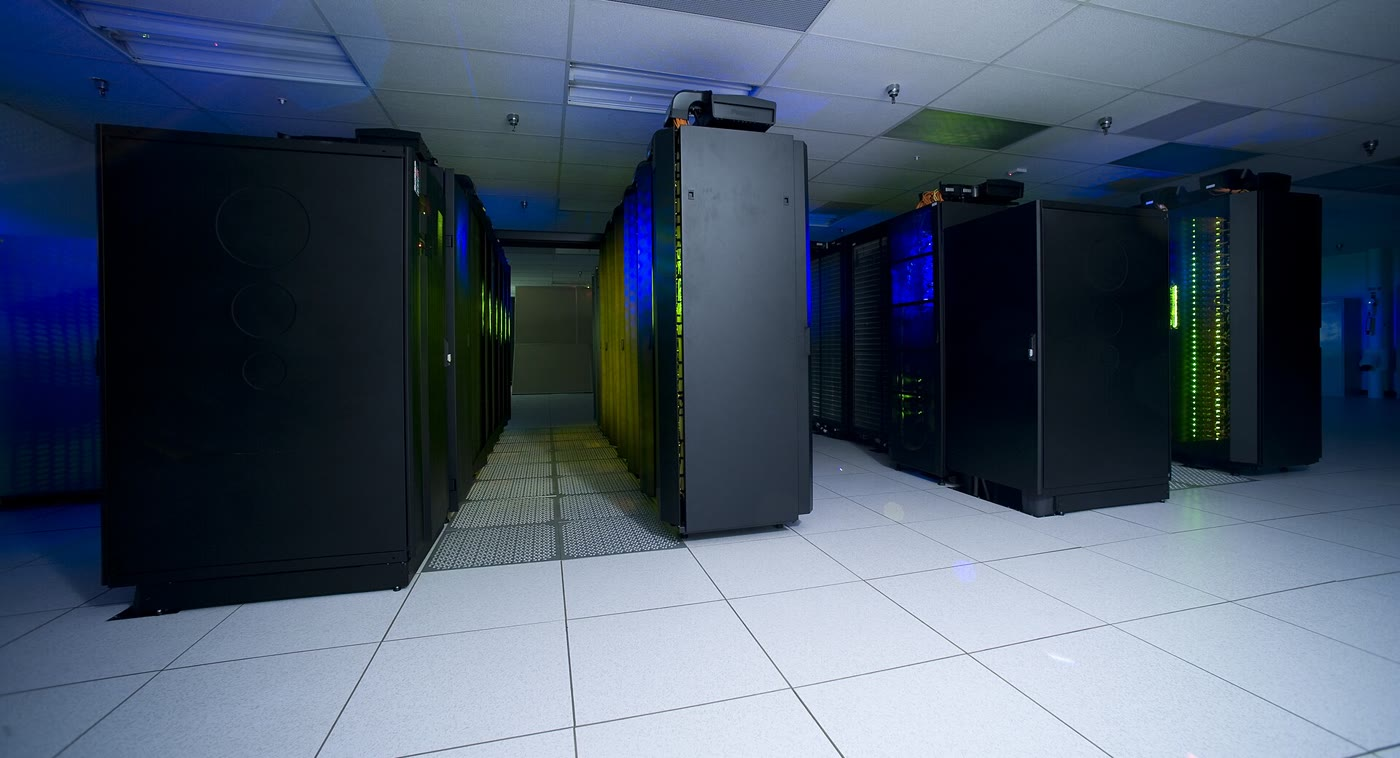
\includegraphics[width=0.7\linewidth]{images/book5/b3-nccs-supercomputer.jpg}

\par\smallskip{\small Armários de um supercomputador no NASA Center for
Climate Simulation, Goddard Space Flight Center, em 2010 (NASA, domínio
público). As equações de um modelo global são resolvidas numericamente em tais
computadores de alto desempenho.}\label{fig:b3:climate-models:supercomputer}
\end{omfigure}
% ledger: photo:b3-nccs, ar6ch1:esm

\section{Avaliação de modelos}\label{sec:b3:climate-models:evaluation}

Um modelo é testado contra o clima observado; o problema é que ele também foi ajustado a esse clima.
Cada \omterm{def:b3:climate-models:gcm}{parametrização} tem parâmetros cuja
faixa aceitável é fixada pela física e pela observação, e, à medida que os componentes
são reunidos, os modeladores os refinam até que o clima simulado atenda a um
conjunto de metas de ajuste: o clima médio --- por exemplo, uma temperatura média
próxima da observada sob a insolação atual --- características regionais, ou
as tendências do período histórico. Só então o modelo é liberado para
as intercomparações.
% ledger: ar6ch1:models, ar6ch1:parameterization, ar6ch1:large-ensembles

\begin{definition}[Projeto de intercomparação de modelos]\label{def:b3:climate-models:cmip}
Um \emph{projeto de intercomparação de modelos}\index{projeto de intercomparação de modelos}
é um conjunto coordenado de experimentos --- os mesmos forçamentos, os
mesmos protocolos, as mesmas saídas --- executado por muitos grupos de modelagem com
seus próprios modelos, de modo que os resultados possam ser comparados. O Coupled Model
Intercomparison Project (CMIP) roda em fases sucessivas; sua sexta fase,
CMIP6, foi uma linha de evidências central da sexta avaliação.
\end{definition}

\begin{dated}{2021}
Dos 29 grupos de modelagem do CMIP6 que relataram como ajustaram seus modelos, 23 não
ajustaram seus modelos ao aquecimento observado no período histórico, e
25 não ajustaram sua ECS: a sensibilidade da maioria dos modelos é uma
propriedade emergente, não um dado de entrada. Em média, os modelos do CMIP6 têm ECS e
TCR maiores que os da fase anterior, e uma dispersão maior que as faixas
avaliadas pelo relatório; em alguns modelos isso foi atribuído à retroalimentação
das nuvens das latitudes médias e altas. Alguns dos modelos mais sensíveis
reproduzem menos bem o aquecimento recente observado e os climas do passado.
A avaliação, portanto, não tirou suas faixas de ECS e TCR diretamente dos
modelos, mas da compreensão dos processos de retroalimentação, do
registro instrumental, dos climas do passado e das restrições emergentes; trata os modelos mais sensíveis como guia para
desfechos de baixa probabilidade e alto impacto (\emph{alta confiança}).
\end{dated}
% ledger: ar6ch1:models, ar6ch7:cmip6-sensitivity

\begin{definition}[Grande conjunto; restrição emergente]\label{def:b3:climate-models:evaluation}
Um \emph{grande conjunto}\index{grande conjunto} é um conjunto de muitas simulações
de um único modelo, com os mesmos forçamentos no mesmo período, que diferem
apenas em seus estados iniciais. Uma \emph{restrição
emergente}\index{restrição emergente} é uma relação, encontrada em um
conjunto de modelos diferentes, entre uma grandeza observável do
clima atual e uma grandeza do clima futuro, como a ECS; o
valor observado da primeira então estreita a faixa da segunda.
\end{definition}

O clima é caótico, de modo que diferenças minúsculas do estado inicial levam os
membros de um \omterm{def:b3:climate-models:evaluation}{grande conjunto} por caminhos diferentes: a dispersão dos
membros mede a variabilidade interna, e sua média, a resposta forçada.
\omterm{def:b3:climate-models:evaluation}{Grandes conjuntos} de vários modelos respaldaram a avaliação. Uma
\omterm{def:b3:climate-models:evaluation}{restrição emergente} precisa de uma razão física. Com algumas dezenas de modelos,
milhares de observáveis podem ser testados, e alguns vão se correlacionar com a
ECS por acaso; a avaliação manteve aqueles com base física, muitos
deles sobre as nuvens dos trópicos, e alertou que um viés compartilhado por todos
os modelos do conjunto anula o método.
% ledger: ar6ch1:large-ensembles, ar6ch7:emergent

\begin{inthelab}[Um centro de modelagem]
\begin{minipage}[t]{0.55\linewidth}\vspace{0pt}
Em um centro de modelagem climática, o modelo é um programa escrito e
mantido por uma equipe: atmosfera, oceano, gelo marinho e continente são componentes
separados, trocando fluxos em suas interfaces por meio de um acoplador. Antes
de uma rodada, os forçamentos do experimento são lidos — as concentrações de
gases de efeito estufa, os aerossóis, o uso da terra previsto no protocolo. O globo é
dividido em pedaços que os processadores do supercomputador calculam lado a
lado, e um século de clima simulado volta na forma de um grande arquivo de
campos. Os cientistas as exibem em telas, comparam-nas com
reanálises e registros de satélite, e enviam as saídas padronizadas ao
arquivo da intercomparação, onde outros grupos as comparam com as suas.
\end{minipage}\hfill
\begin{minipage}[t]{0.42\linewidth}\vspace{0pt}
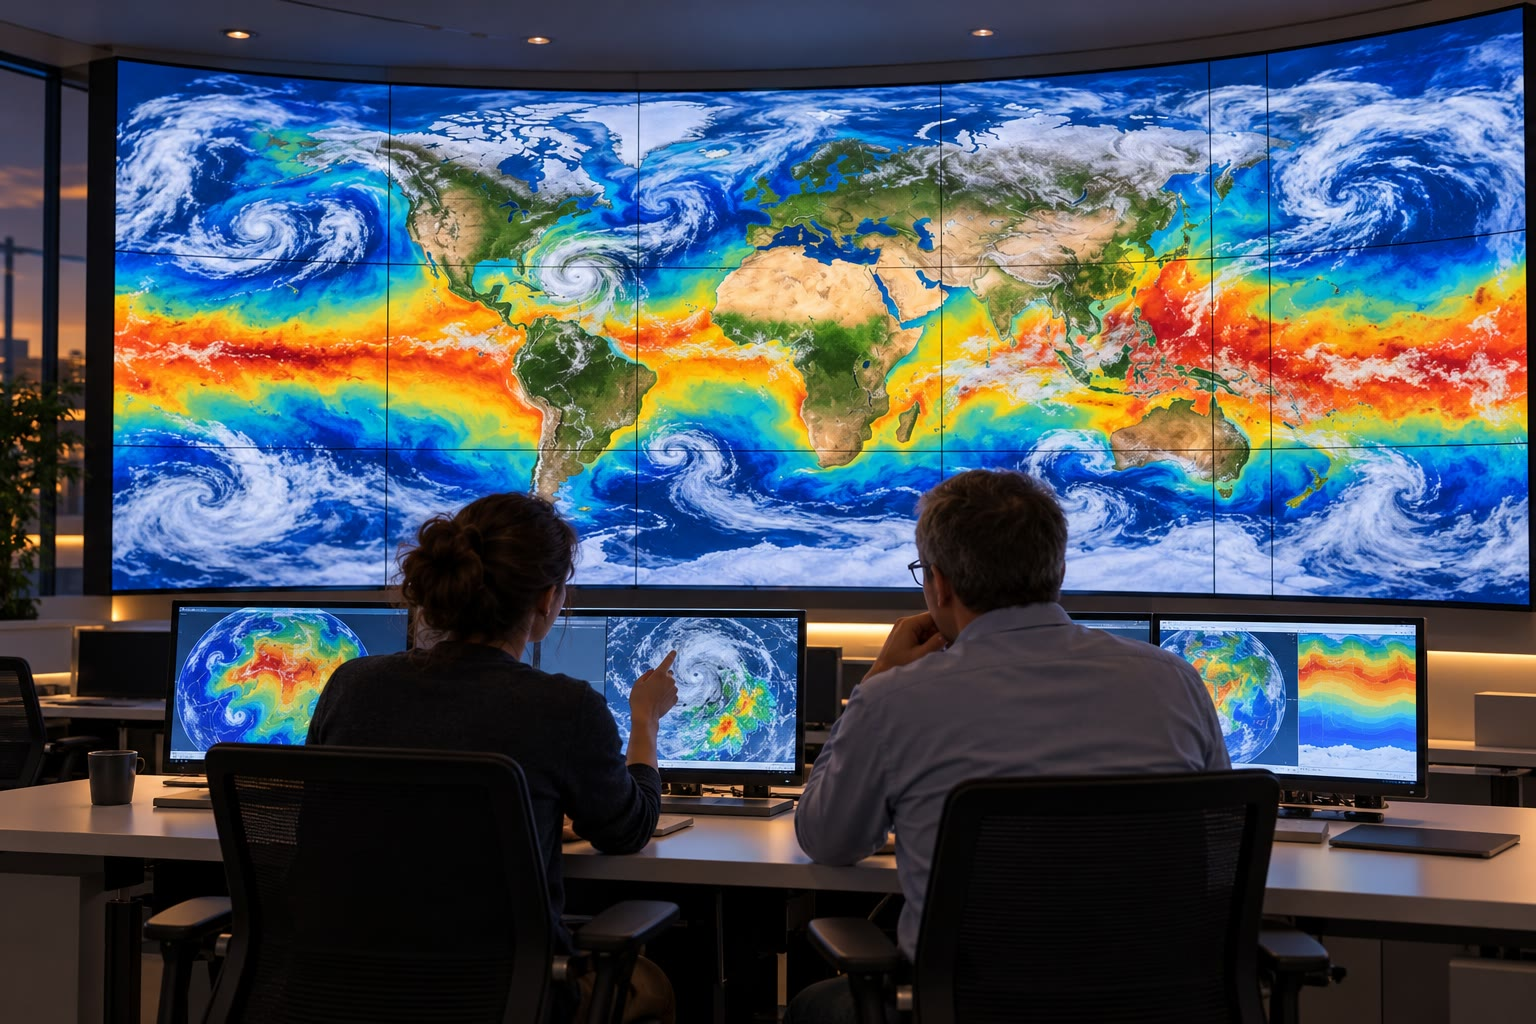
\includegraphics[width=\linewidth]{images/book5/ai/b3-model-centre.jpg}

{\scriptsize Dois cientistas diante de uma parede de telas mostrando campos globais
de uma rodada do modelo. Ilustração gerada por IA.}
\end{minipage}
\end{inthelab}
% ledger: ar6ch1:esm, ar6ch1:models

\section{Exercícios}

\begin{exercise}[$\star$]\label{exo:b3:climate-models:1}
A lei de OLR de Budyko é $I = a + bT - (a_1 + b_1T)n$, com $a = 14.0$, $b =
0.14$, $a_1 = 3.0$, $b_1 = 0.10$, em \unit{kcal.cm^{-2}} por mês e $T$
em \unit{\celsius}. Para uma nebulosidade $n = 0.5$, calcule $A$ e $B$, e
converta-os para \unit{W/m^2} e \unit{W.m^{-2}.\celsius^{-1}}, com um
mês igual a um doze avos de um ano de 365.25 dias. Qual OLR a lei fornece a
\qty{15}{\celsius}?
\end{exercise}
% ledger: budyko69:olr

\begin{exercise}[$\star$]\label{exo:b3:climate-models:2}
Com $Q = \qty{340}{W/m^2}$, $A = \qty{211.9}{W/m^2}$ e $B =
\qty{1.816}{W.m^{-2}.\celsius^{-1}}$, calcule a temperatura de equilíbrio
para um albedo de 0.30 e de 0.31. De quanto um aumento de 0.01 do
albedo resfria este planeta?
\end{exercise}

\begin{exercise}[$\star$]\label{exo:b3:climate-models:3}
Calcule a capacidade térmica por metro quadrado de uma camada misturada de água do mar
com \qty{60}{m} de profundidade, $\rho = \qty{1025}{kg/m^3}$ e $c_p = \qty{3992}{J.kg^{-1}.K^{-1}}$,
em \unit{J.m^{-2}.K^{-1}} e em \unit{W.yr.m^{-2}.K^{-1}}. Calcule o
tempo de resposta do \cref{thm:b3:climate-models:response} para $\lambda = -B =
\qty{-1.816}{W.m^{-2}.\celsius^{-1}}$ e para $\lambda =
\qty{-1.33}{W.m^{-2}.\celsius^{-1}}$.
\end{exercise}
% ledger: teos10:cp0

\begin{exercise}[$\star$]\label{exo:b3:climate-models:4}
Para o modelo de duas camadas com $\lambda = \qty{-1.33}{W.m^{-2}.\celsius^{-1}}$,
$\gamma = \qty{0.62}{W.m^{-2}.\celsius^{-1}}$ e $F_{2\times} =
\qty{3.93}{W/m^2}$, calcule a ECS, o TCR aproximado $F_{2\times}/
(\gamma - \lambda)$, e a razão entre elas.
\end{exercise}
% ledger: ar6sm7:two-layer, ipcc:erf-2xco2

\begin{exercise}[$\star\star$]\label{exo:b3:climate-models:5}
No modelo zero-dimensional do texto, considere uma constante solar de
\qty{1340}{W/m^2}. Encontre os três equilíbrios e a inclinação $N'(T)$ do
fluxo líquido em cada um; quais são estáveis?
\end{exercise}

\begin{exercise}[$\star\star$]\label{exo:b3:climate-models:6}
Desloque a rampa de albedo do texto: $\alpha = 0.62$ abaixo de \qty{-20}{\celsius},
$0.30$ acima de \qty{0}{\celsius}, linear entre os dois. Mantenha $A$ e $B$. Para qual
constante solar o ramo quente termina, e em quantos por cento isso fica
abaixo de \qty{1360}{W/m^2}? Para qual constante solar a bola de neve derrete?
O que determina o tamanho do limiar?
\end{exercise}

\begin{exercise}[$\star\star$]\label{exo:b3:climate-models:7}
Um planeta-modelo com os parâmetros do texto está no estado de bola de neve.
(a)~Qual é a sua temperatura com a constante solar atual? (b)~Mantendo o Sol
como está, qual forçamento $F$ elevaria a temperatura da bola de neve até
\qty{-10}{\celsius}? Quantas vezes ele vale o forçamento de uma duplicação do
dióxido de carbono, \qty{3.93}{W/m^2}? (c)~Uma vez que o gelo tenha desaparecido, para onde o planeta
se estabiliza quando o forçamento é então removido?
\end{exercise}
% ledger: ipcc:erf-2xco2, hoffman17:hysteresis

\begin{exercise}[$\star\star$]\label{exo:b3:climate-models:8}
O modelo X, um modelo de duas camadas inventado, tem $C = 7.0$ e $C_d =
\qty{90}{W.yr.m^{-2}.\celsius^{-1}}$, $\gamma = 0.70$ e $\lambda =
\qty{-1.10}{W.m^{-2}.\celsius^{-1}}$. Calcule suas duas escalas de tempo exatamente
e com as aproximações do \cref{thm:b3:climate-models:two-layer}, a
fração $a_f$, sua ECS e seu TCR aproximado.
\end{exercise}

\begin{exercise}[$\star\star$]\label{exo:b3:climate-models:9}
No modelo de Budyko do texto, $\bar T = \qty{12.81}{\celsius}$, $\beta =
\qty{3.74}{W.m^{-2}.\celsius^{-1}}$, a linha de gelo em \ang{72}, $s = 1.221$
no equador e $0.506$ no polo, $\alpha = 0.30$ e $0.62$.
Calcule a temperatura no equador e no polo, e o calor
$\beta(T - \bar T)$ que o transporte retira de, ou traz para, cada
metro quadrado ali.
\end{exercise}

\begin{exercise}[$\star\star\star$]\label{exo:b3:climate-models:10}
Um planeta sem gelo ($\alpha = 0.30$ em toda parte) tem o
transporte difusivo $D = -\mathcal D\,\partial_x[(1 - x^2)\partial_xT]$ e a
insolação $s(x) = 1 + s_2P_2(x)$, $P_2 = (3x^2 - 1)/2$. (a)~Mostre que
$\partial_x[(1 - x^2)\partial_xP_2] = -6P_2$. (b)~Mostre que $T = T_0 +
T_2P_2(x)$ é uma solução estacionária, com $T_0 = (Q(1 - \alpha) - A)/B$ e
$T_2 = Qs_2(1 - \alpha)/(B + 6\mathcal D)$. (c)~A insolação da
reanálise dá $s_2 = \num{-0.476}$. Sem transporte, qual seria a
diferença de temperatura entre equador e polo? (d)~Qual $\mathcal D$ fornece
a diferença observada, \qty{55.3}{\celsius}?
\end{exercise}
% ledger: data:b3-ncep, data:b5-ncep-air

\begin{exercise}[$\star\star\star$]\label{exo:b3:climate-models:11}
(a)~Escreva a quadrática do \cref{thm:b3:climate-models:two-layer} como $r^2 -
\Sigma r + \Pi = 0$ e mostre que, se $4\Pi \ll \Sigma^2$, suas raízes são
próximas de $\Sigma$ e de $\Pi/\Sigma$. (b)~Para um forçamento $F = kt$ crescendo
linearmente, mostre que, uma vez que $t \gg \tau_f$, e enquanto $T_d$ permanecer pequeno,
$T \approx kt/(\gamma - \lambda)$; deduza o TCR aproximado. (c)~Verifique
os números do texto: $\Sigma$, $\Pi$, as duas escalas de tempo e a
razão $4\Pi/\Sigma^2$.
\end{exercise}
% ledger: ar6sm7:two-layer

\begin{exercise}[$\star\star\star$]\label{exo:b3:climate-models:12}
Um conjunto inventado de oito modelos fornece um observável $X$ do
clima atual e suas ECS:
\begin{center}
\begin{tabular}{l*{8}{c}}
\hline
$X$ & 0.2 & 0.5 & 0.6 & 0.8 & 1.0 & 1.1 & 1.3 & 1.5\\
ECS (\unit{\celsius}) & 2.3 & 2.7 & 3.1 & 3.2 & 3.8 & 3.9 & 4.4 & 4.6\\
\hline
\end{tabular}
\end{center}
(a)~Calcule a média e o desvio-padrão da ECS do
conjunto. (b)~Ajuste ECS $= a + bX$ por mínimos quadrados; calcule a correlação
e o desvio-padrão dos resíduos. (c)~O $X$ observado é $0.7
\pm 0.1$. Qual ECS a restrição fornece, e com que dispersão?
(d)~O que o faria desconfiar dessa restrição?
\end{exercise}
% ledger: ar6ch7:emergent

\section{Problema: quão perto de uma bola de neve?}

\begin{problem}[{Problema de fim de semana --- equilíbrios, estabilidade e o
limiar de glaciação de um planeta modelo}]
\label{pb:b3:climate-models:1}
Um planeta modelo tem a constante solar de hoje $S_0 = \qty{1360}{W/m^2}$ e a
lei da OLR $A + BT$, com $A = \qty{211.9}{W/m^2}$ e $B =
\qty{1.816}{W.m^{-2}.\celsius^{-1}}$. Seu albedo é 0.62 abaixo de
\qty{-10}{\celsius}, 0.30 acima de \qty{+10}{\celsius}, com variação linear entre esses valores, e
sua capacidade térmica superficial $C = \qty{8.1}{W.yr.m^{-2}.\celsius^{-1}}$. Considere
$\sigma = \qty{5.670e-8}{W.m^{-2}.K^{-4}}$.

\medskip\noindent\textbf{Parte I --- O planeta em equilíbrio.}
\begin{enumerate}
\item Calcule a insolação média $Q_0$ por metro quadrado do planeta, e
  explique o fator.
\item Calcule a insolação absorvida com albedo de 0.30, e a OLR a
  \qty{15}{\celsius}.
\item Calcule o equilíbrio quente.
\item Calcule o equilíbrio de bola de neve, e verifique que ele está no
  ramo gelado.
\item Calcule o terceiro equilíbrio, sobre a rampa de albedo.
\item Calcule a temperatura de emissão que devolve ao espaço, como corpo negro, a insolação absorvida
  e compare-a com o equilíbrio quente.
\end{enumerate}

\medskip\noindent\textbf{Parte II --- Estabilidade e tempo.}
\begin{enumerate}[resume]
\item Calcule a inclinação $N'(T)$ do fluxo líquido em cada equilíbrio, e diga
  quais são estáveis.
\item Um pequeno afastamento do equilíbrio intermediário cresce como $\mathrm
  e^{t/\tau}$. Calcule $\tau$.
\item Calcule o tempo de resposta do equilíbrio quente.
\item Um forçamento de \qty{3.93}{W/m^2}, o de uma duplicação do dióxido de carbono,
  é ativado. Calcule o aquecimento em equilíbrio e compare-o com
  a ECS avaliada para o clima real.
\item Quanto tempo o modelo leva para cobrir \qty{95}{\percent} do
  aquecimento? Por que o clima real leva mais tempo?
\end{enumerate}

\medskip\noindent\textbf{Parte III --- A bifurcação sela-nó.}
\begin{enumerate}[resume]
\item À medida que o Sol enfraquece, em que temperatura o equilíbrio quente encontra
  o intermediário? Calcule $Q$ nesse ponto.
\item Calcule a constante solar na bifurcação, e a queda em relação a
  hoje, em por cento.
\item Logo abaixo dela, para onde vai o clima? Calcule sua temperatura.
\item Calcule a constante solar em que a bola de neve derrete, e o aumento em relação a
  hoje, em por cento.
\item Esboce o laço percorrido pela temperatura quando $S_0$ é reduzida
  abaixo da bifurcação e trazida de volta a \qty{1360}{W/m^2}.
\end{enumerate}

\medskip\noindent\textbf{Parte IV --- A linha de gelo.} Dê ao planeta
o modelo latitudinal de Budyko, com $\beta = \qty{3.739}{W.m^{-2}.\celsius^{-1}}$,
um albedo de gelo de 0.62 no lado polar da linha de gelo, 0.30 no lado equatorial, 0.50 na
borda, e a insolação da reanálise:
\begin{center}
\begin{tabular}{lccccccc}
\hline
latitude & \ang{0} & \ang{30} & \ang{40} & \ang{47.5} & \ang{55} & \ang{60} & \ang{72}\\
$s(x_s)$ & 1.2211 & 1.0730 & 0.9647 & 0.8688 & 0.7650 & 0.6947 & 0.5643\\
$F(x_s)$ & 0 & 0.5865 & 0.7324 & 0.8192 & 0.8863 & 0.9205 & 0.9738\\
\hline
\end{tabular}
\end{center}
\begin{enumerate}[resume]
\item Com a linha de gelo em \ang{72}, calcule o albedo médio $\bar\alpha$
  e a temperatura média $\bar T$.
\item Calcule a temperatura crítica $T_c$ que coloca a borda em
  \ang{72} hoje, e compare-a com a reanálise, \qty{-15.8}{\celsius}.
\item Calcule o numerador de $Q(x_s)$ na \cref{prop:b3:climate-models:iceline}
  e a razão $\beta/B$.
\item Calcule $Q(x_s)/Q_0$ para a linha de gelo em \ang{30}, \ang{40},
  \ang{47.5}, \ang{55} e \ang{60}.
\item Onde está o mínimo desses valores? Quais linhas de gelo são estáveis?
\item Com o Sol de hoje, que outra linha de gelo o modelo permite, e ela é
  estável? A bola de neve é possível hoje? (Use a coluna \ang{0}.)
\item Compare o limiar do modelo latitudinal com o da Parte~III
  e com o de Budyko, \qty{1.6}{\percent}, e a latitude do gelo no
  limiar com a dele, \ang{50}.
\item Dê, com dois algarismos significativos, a queda da constante solar, em
  por cento, que glaciaria o planeta modelo.
\end{enumerate}
\end{problem}
% ledger: nasa:solar-mean, data:b5-ncep-air, data:b3-ncep, budyko69:transport, budyko69:albedo, budyko69:threshold, ipcc:ecs, const:sigma
